\newcommand{\figureLCDCharPlayerJump}[1]{
  \def\lang{\detokenize{#1}}
  \def\langRu{\detokenize{ru}}
  \def\langEn{\detokenize{en}}
  \def\figureCaption{XXX: No translation.}
  \ifx \lang\langRu
  \def\figureCaption{
    Анимация прыжка игрока.
  }
  \fi
  \ifx \lang\langEn
  \def\figureCaption{
    Player jump animation.
  }
  \fi
  \begin{figure}[ht]
    \centering
    \def \offsetJump{0.0}
    \def \offsetSquat{3.5}
    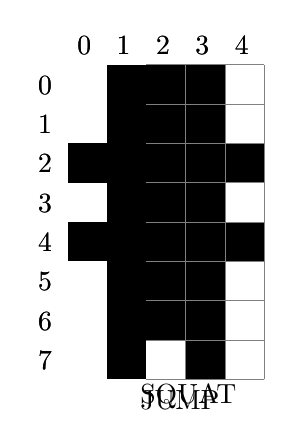
\begin{tikzpicture}
      %% Jump.
      %% 0
      \fill[black] (\offsetJump + 2.0, 0) rectangle (\offsetJump + 0.5, -1.0);
      %% 2
      \fill[black] (\offsetJump + 2.0, -1.0) rectangle (\offsetJump + 2.5, -1.5);
      \fill[black] (\offsetJump + 1.0, -1.0) rectangle (\offsetJump + 1.5, -1.5);
      \fill[black] (\offsetJump + 0.5, -1.0) rectangle (\offsetJump + 0.0, -1.5);
      %% 3
      \fill[black] (\offsetJump + 0.5, -1.5) rectangle (\offsetJump + 2.0, -2.0);
      %% 4
      \fill[black] (\offsetJump + 1.5, -2.0) rectangle (\offsetJump + 1.0, -2.5);
      %% 5
      \fill[black] (\offsetJump + 0.5, -2.5) rectangle (\offsetJump + 2.0, -3.0);
      %% 6
      \fill[black] (\offsetJump + 2.0, -3.0) rectangle (\offsetJump + 1.5, -3.5);
      \fill[black] (\offsetJump + 1.0, -3.0) rectangle (\offsetJump + 0.5, -3.5);
      %% 7
      \fill[black] (\offsetJump + 2.0, -3.5) rectangle (\offsetJump + 1.5, -4.0);
      \fill[black] (\offsetJump + 1.0, -3.5) rectangle (\offsetJump + 0.5, -4.0);

      \draw[step=0.5cm,gray,very thin] (\offsetJump, -4.0) grid (\offsetJump + 2.5, 0);
      %% Numbers
      \foreach[count=\n from 0] \x in {0.0, 0.5, ..., 2.0} {
        \draw (\offsetJump + \x, 0) node[anchor=south west] {$\n$};
      }
      \foreach[count=\n from 0] \y in {-0.5, -1.0, ..., -4.0} {
        \draw (\offsetJump - 0.5, \y ) node[anchor=south west] {$\n$};
      }
      \draw (\offsetJump + 0.8, -4.5) node[anchor=south west] {JUMP};

      %% Squat.
      %% 0
      %% 1
      \fill[black] (\offsetSquat + 0.5, -0.5) rectangle (\offsetSquat + 2.0, -1.5);
      %% 3
      \fill[black] (\offsetSquat + 1.0, -1.5) rectangle (\offsetSquat + 1.5, -2.0);
      %% 4
      \fill[black] (\offsetSquat + 0.0, -2.0) rectangle (\offsetSquat + 2.5, -2.5);
      %% 4
      \fill[black] (\offsetSquat + 1.0, -2.5) rectangle (\offsetSquat + 1.5, -3.0);
      %% 5
      \fill[black] (\offsetSquat + 0.5, -3.0) rectangle (\offsetSquat + 2.0, -3.5);
      %% 6
      \fill[black] (\offsetSquat + 0.5, -3.5) rectangle (\offsetSquat + 1.0, -4.0);
      \fill[black] (\offsetSquat + 1.5, -3.5) rectangle (\offsetSquat + 2.0, -4.0);

      \draw[step=0.5cm,gray,very thin] (\offsetSquat, -4.0) grid (\offsetSquat + 2.5, 0);
      %% Numbers
      \foreach[count=\n from 0] \x in {0.0, 0.5, ..., 2.0} {
        \draw (\offsetSquat + \x, 0) node[anchor=south west] {$\n$};
      }
      \foreach[count=\n from 0] \y in {-0.5, -1.0, ..., -4.0} {
        \draw (\offsetSquat - 0.5, \y) node[anchor=south west] {$\n$};
      }
      \draw (\offsetSquat + 0.8, -4.5) node[anchor=south west] {SQUAT};
    \end{tikzpicture}
    \caption{\figureCaption}
    \label{fig:game-dev-player-textures}
  \end{figure}
}
